\documentclass[11pt]{article}
\usepackage[
  left=1in,
  right=1in,
  top=0.5in,
  bottom=0.8in
]{geometry}
% \usepackage{fullpage}
\usepackage{graphicx}
\usepackage{biblatex}
\addbibresource{export.bib}

\begin{document}

\title{ARMv8 AArch64 Project Final Report}
\author{Constantin Filip, Daniel Howard, Maximillian Smith, Vladimir Filip}

\maketitle

\section{Assembler Structure and Implementation}
Our assembler consists of the following components:
\begin{itemize}
    \item A tokeniser for converting each line of assembly code into a sequence of tokens describing the kind of token and its contents
    \item A parser for converting tokens into an internal representation (IR)
    \item A symbol table storing the address of labels
    \item A collection of binary generation functions, each of which converts the IR of a single instruction to binary.
\end{itemize}
The assembler is two-pass as each source code line is traversed twice, first in plaintext, and then in its IR. The IR struct contains a nested union coupled with a pointer to a function that converts that instance of the IR to its corresponding binary form. The members of the union represent the different types of instruction. We did not include any flags to indicate what type of instruction a particular instance encodes, as it was left to the parser to populate the union correctly and set the function pointer to the correct \texttt{toBinary} function, which assumes that the variables are set correctly as a precondition.

Directives are handled as instructions whose binary representation is the integer value in the source code declaration. During parsing, the sequence of tokens for aliases are converting into the corresponding alias and parsed as normal.

Overall, the assembler implementation was substantial due of the collection of functions and the initialisation code for a hashmap linking each function for both stages. While the assembler has a sophisticated tokeniser and error handling, these features complicated the design of the assembler beyond the requirements of the specification.

\section{LED Blink Implementation}

After reading the specification's documentation on how to interact with the pi's GPIO pins, we decided on a pin to connect the LED to. We did this because there was no need to make the connecting pin variable, so hard-coding the values to address the pins made the assembly simpler. We chose pin 2, making the \texttt{GPFSEL}, \texttt{GPSET} and \texttt{GPCLR} addresses \texttt{0x3f20 0000}, \texttt{0x3f20 001c} and \texttt{0x3f20 0028}, respectively. We noticed that \texttt{GPSET} and \texttt{GPCLR} can be calculated by \texttt{orr}-ing  \texttt{GPFSEL} with \texttt{0x001c} and \texttt{0x0028} respectively, meaning we could set the value \texttt{0x3f20} once (with \texttt{lsl \#16} and \texttt{movz} to ensure the rest of the register was \texttt{0}).

We also calculated that for pin 2, we had to set the \texttt{GPFSEL} register to \texttt{0x0040} to set it as an output pin and the \texttt{GPSET} and \texttt{GPCLR} registers to \texttt{0x0004} to set and clear the output.

We decided to use one register per value to make the assembly easier to read, \texttt{w0} stores the address of \texttt{GPFSEL}, \texttt{w1} stores the value that must be written to \texttt{GPFSEL}, \texttt{w2} stores the address of \texttt{GPSET}, \texttt{w3} stores the address of \texttt{GPCLR} and \texttt{w4} stores the value that must be written to \texttt{GPSET} or \texttt{GPCLR}.

Once the pin was configured, we started looping logic, starting with a counter limit value stored in \texttt{x5}, initially set to \texttt{0xffff} with the ability to go back later and choose a better value. We then enable the output from pin 2 by setting the \texttt{GPSET} register to the value in \texttt{w4}, this operation was labeled with \texttt{on} so it can be branched back to later. \texttt{x6} then stores a counter starting at \texttt{0}, this is incremented in a loop until the value in \texttt{x5} equals the value in \texttt{x6}. Then the \texttt{GPCLR} register is set to the value in \texttt{w4}. We then reset the counter and loop once again until it reaches \texttt{x5}. We then branch back to the label mentioned previously.

After running for the first time, we found that the LED stayed on without turning off, we suspected that this may be because of our counter value being too low, so we changed it to \texttt{0x003f ffff} and found that this value produced a good flashing speed.

\section{Extension - Distributed Database}

\subsection{Overview}

Our goal was to build a fault-tolerant distributed database that is BASE (Basically Available Soft state Eventually consistent) instead of the standard ACID database system \cite{RefWorks:2025acid}.
We used the Raft algorithm to maintain consensus between nodes in a performant manner, assuming that $\lfloor\frac{n}{2}\rfloor + 1$ remain nodes online at all times, where $n$ is the number of nodes in the system \cite{RefWorks:ongaro2014search}.
Our system has an SQL-inspired JSON query syntax. The operations that can be performed on the database are SELECT, INSERT, UPDATE, DELETE and CREATE TABLE.

A database designed like this can be used anywhere where stale reads are allowed. The database should not be used in any situation where data must always be consistent everywhere as the Raft algorithm is not designed to do this. A good application of this database would be a messaging service like Discord, where there are many more reads than writes (as every node can handle reads), and temporarily stale reads are acceptable.

\subsection{High Level Design}

We made an initial design of how each node would work so that we could split up the work of implementing it. The initial design can be seen in: Figure \ref{InitialNodeDesign}.

\begin{figure}[ht]
    \centering
    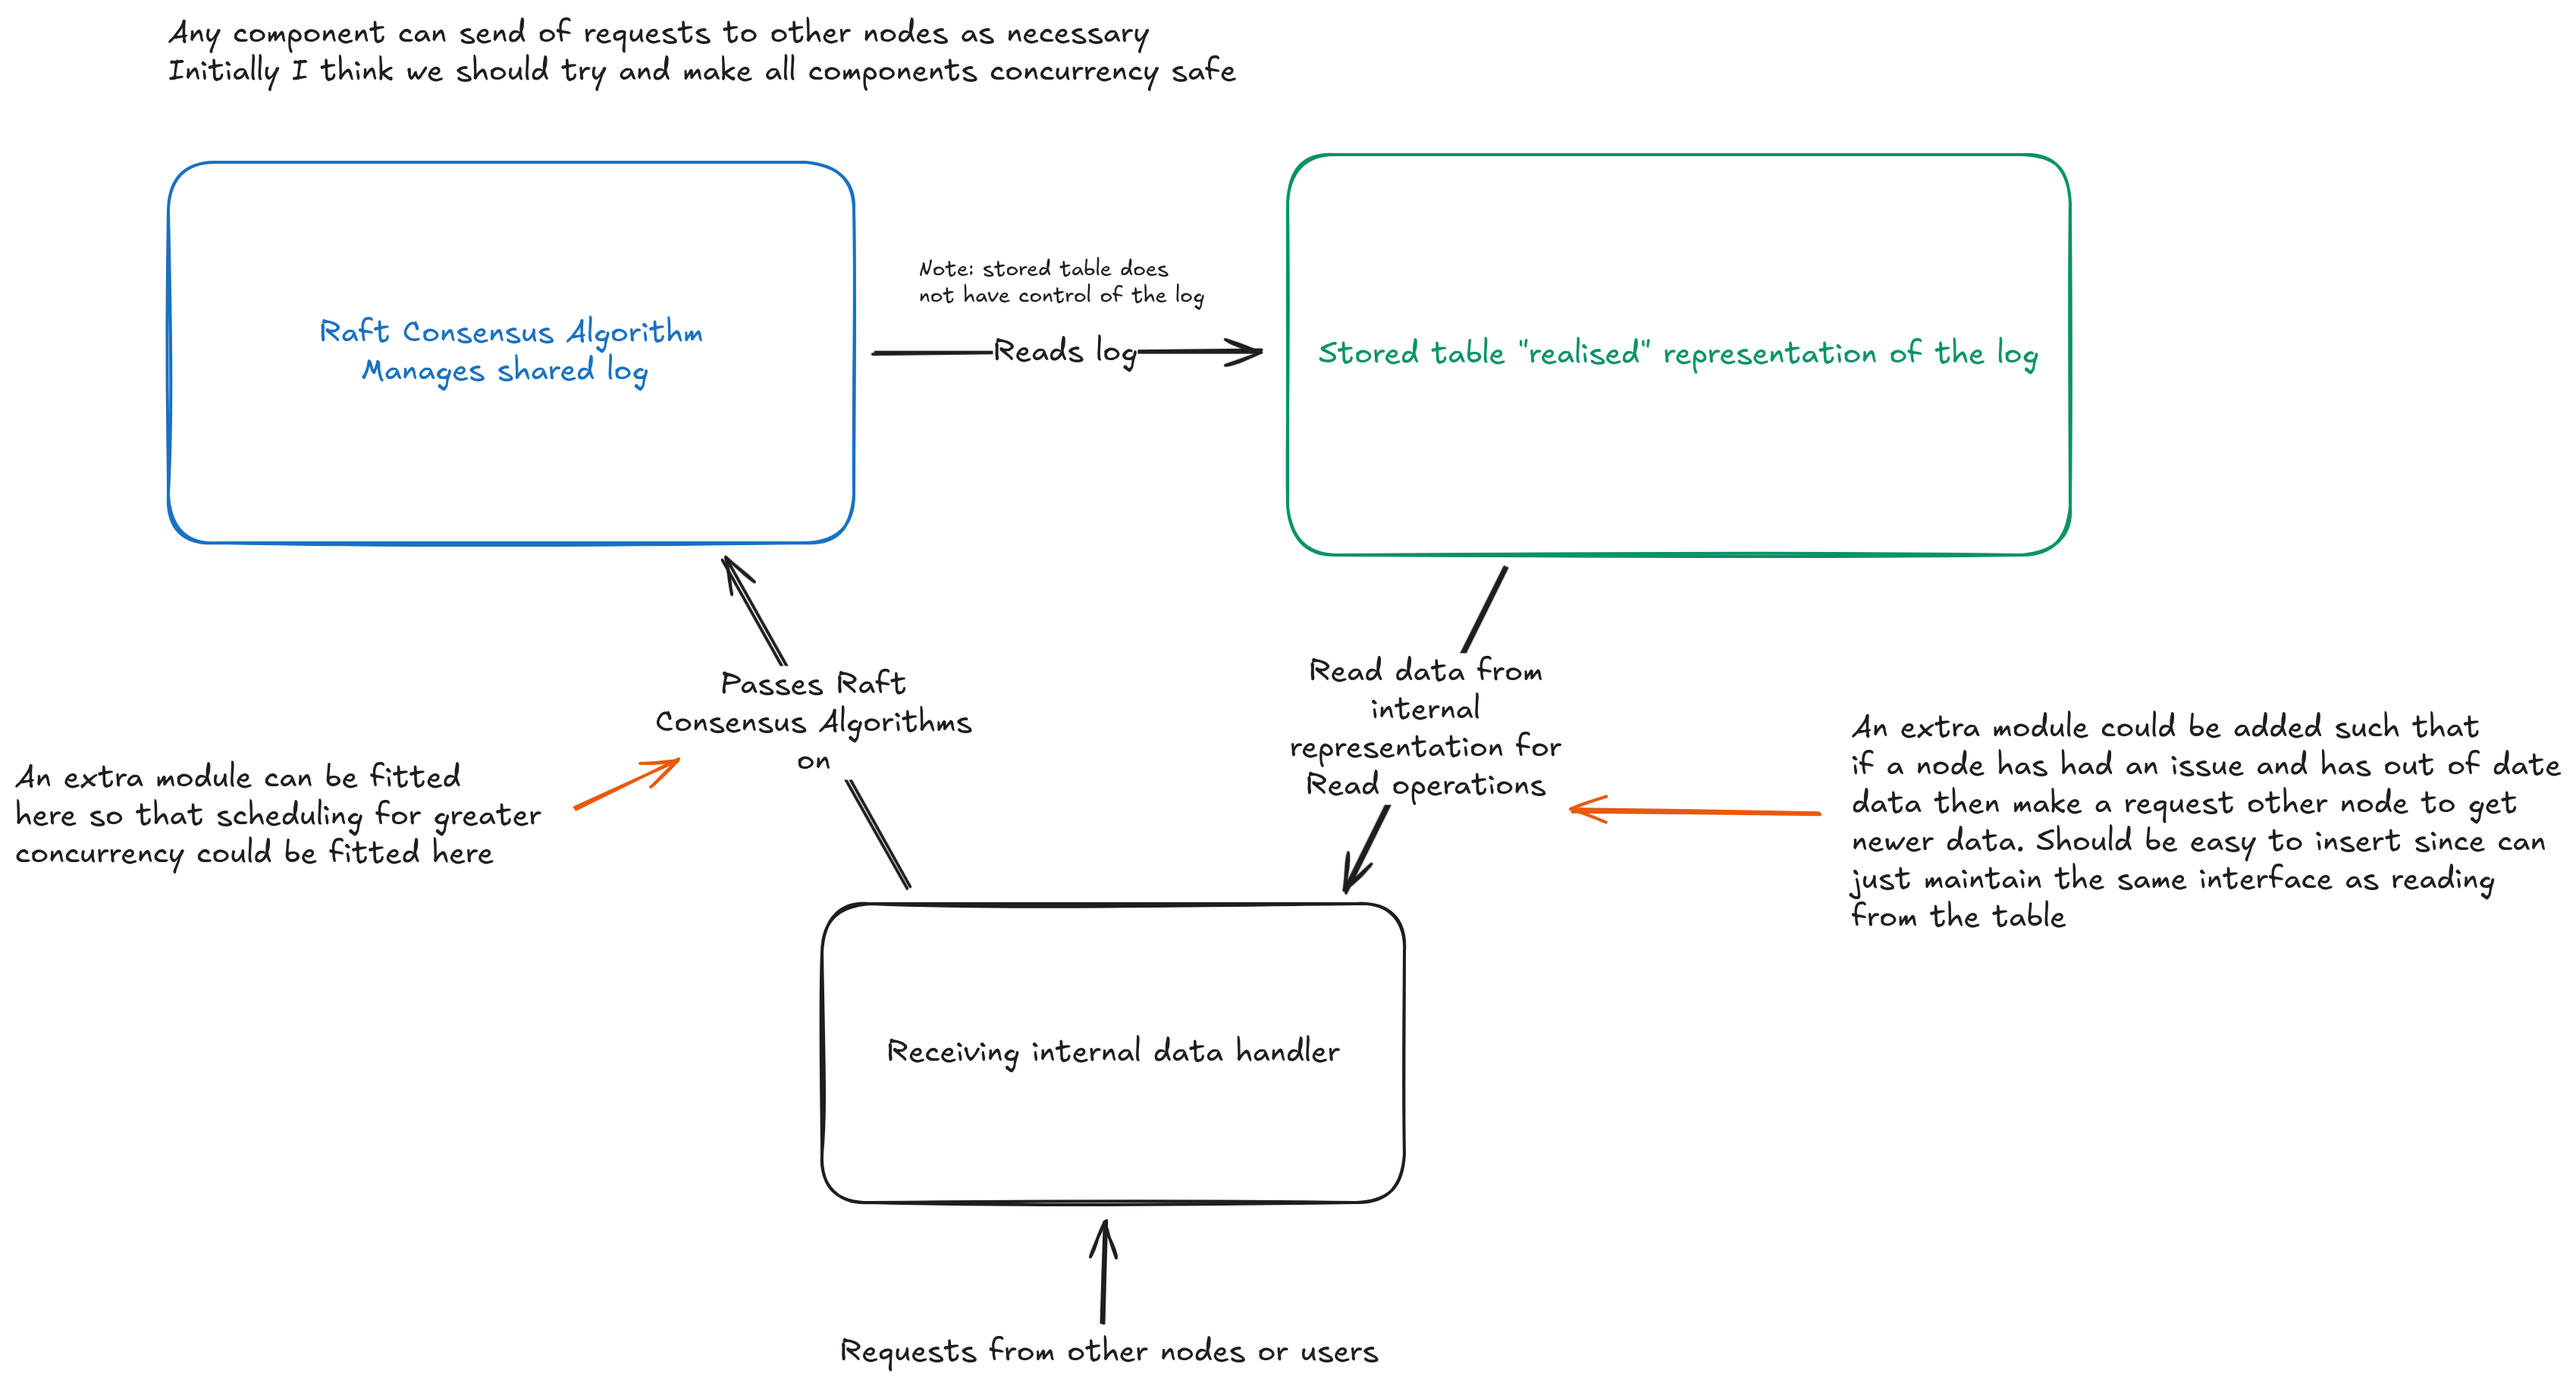
\includegraphics[width=0.75\linewidth]{InitialNodeDesign.png}
    \caption{Initial Internal Node Structure}
    \label{InitialNodeDesign}
\end{figure}

We split the work into three main areas: networking, Raft distributed algorithm and data storage. We initially designed how the sections would interact. We did this to enable us to work without having to deal with tightly coupled code. This resulted in quickly developing working components which we could then combine.

\subsubsection{Networking}

We originally planned to have each node running a basic TCP server, then every node would connect to each other's servers, however we quickly realised that this created two connections between each node which is unneeded and excessive. To solve this and only have one connection between each node, we said that each node is a client (connects) to nodes with an id less than its own id and would provide a server (get connected to) for nodes with an id greater than its own id. These servers were all implemented using basic OS system calls. With the nature of this project, we also needed the nodes to have the ability to disconnect and reconnect from each other without having to restart the program, this was implemented with a basic reconnect sequence. Each node's connection is handled in a separate thread allowing for a good degree of parallelism. The first message sent between nodes is an identify message to ensure the correct id was given when the server was booted, this adds an extra check to ensure we avoid seeing undetermined side effects from incorrect input.

A major problem we faced with the network was how to handle network failures. We found that the OS is unaware when it looses a network connection, this meant that each node believed that the broken node was still online. We fixed this by adding ping messages (separate to raft's append entry heartbeats), a ping is sent every second, and if a node hasn't received a ping after 5 seconds, it kills its thread and kills the connection to the node, starting the reconnecting sequence again.

Another part of the networks was working out what format to send data across the network in, we settled on encoding all messages in binary, setting all their values sequentially. To handle variable length messages, the size of any variable length structure (like arrays) was stored first, followed by the data itself.

The final part of networking was the connection between a client and each node, we settled on a HTTP server, transferring data using JSON, we chose this to make the database usable in a large number of established applications.

In order to test the networking, we made a \texttt{networkingtest} program, which redefines the \texttt{execute} function to log any data it recieves. We could then run one node in \texttt{gdb} and manually send data, ensuring the correct data was recieved on the other end.

\subsubsection{Raft Consensus Algorithm}

In the Raft algorithm, developed by Diego Ongaro and John Ousterhout \cite{RefWorks:ongaro2014search}, all nodes consist of a log detailing the write operations carried out and an internal state machine. In our case, the state machine is a custom-made database. The behaviour of Raft can be separated into two main sections: leadership elections and handling additions to the log.

In Raft there is a leader node that acts as the `source of truth' among the rest of the nodes. If the leader node exists, it will send heartbeat signals to all other nodes that asserts its authority as the leader. Each node has an election timeout for which if it does not receive a heartbeat, it will call an election and put itself forward as a candidate.
Then there is a voting process, which will select the next leader out of all the candidates for the next term. The quality of a candidate is judged by the term of its last log entry term and index. A candidate declares itself a leader once it has received votes from a majority of the nodes. In each election only one node can be elected leader since each node can only vote once in an election and there cannot be two disjoint majorities of nodes.
Elections can time out if a new leader is not elected within the election timeout, which then causes another election to be called. Each node has a different election timeout (randomised within a set range) so that nodes do not declare an election at the same time.

All write operations are handled by the leader. The leader node appends the write operation to its log, and informs all its followers to append to their logs. Once the leader determines that a majority of the nodes have appended the entry to their logs, it will commit the entry (apply the write operation to the internal database) and inform the followers to do the same.

Read operations can be handled by any node. Even though this may happen before the latest write operations have been committed in all online nodes, Raft ensures that these will eventually be reflected, so the `Eventually Consistent` requirement is met.

This process ensures general consensus on what is the correct log and ensures the distributed database is BASE compliant.

Debugging was the hardest part about implementing the raft algorithm. Using \texttt{gdb} was extremely difficult due to the time dependency of the algorithm, i.e. if we hit a breakpoint the node would not stay a leader as other nodes would call elections. This meant that we had to rely on logging for solving issues. Segmentation faults were still resolved with \texttt{gdb}.

During development, there were issues around nodes calling elections at the same time, in which nodes would have only 1 vote (from themselves), so no leader would ever be elected. This was because our election timeouts were not randomised within a large enough range. We eventually settled on a range of 150-1150ms. The initial code for setting the commit index of followers was also vulnerable to bugs, because of the edge case where the commit index of the leader may be larger than the size of the log of the follower if the follower is significantly out of date. This was solved by setting the follower commit index to the minimum of the leader commit index and the index of the last log entry appended to it.

\subsubsection{Data Storage}

The database supports table creation and selections, insertions, updates and deletions within a single table, with support for variable length records. Each table is stored in its own data file, with its records organised in separate 4KiB pages; storing records in this way maximises spacial locality when iterating through and accessing records, reducing the number of disk accesses.

To support the storage of records which can have variable-length fields, the records are organised in a \textit{slotted page structure} \cite{RefWorks:silberschatz2011database}. Each page contains a header consisting of an array of \textit{slots}, where each slot is a tuple storing the offset and size of the record within the page. Importantly, the position of the slot for a particular record does not change, allowing records to be stored contiguously by shifting records to remove empty spaces (introduced by delete operations) while only updating the offset of its corresponding slot. Additionally, a \(B^+\)-tree index (\(B^+\)-tree index not implemented) could maintain a constant indirect pointer to a record which does not need to be changed when another record is inserted in the same page.

Each data file has accompanying schema and space inventory table. The schema, or data dictionary, stores the type, size and name of each attribute in the table, and is used to interpret and parse raw records in the data file into an record internal representation. The space inventory stores the amount of free space for each page, allowing a page with sufficient free space to be located efficiently during an insertion, especially using a hash index (hash index not implemented). To facilitate their access, creation and modification, the schema and space inventory are themselves stored using the same file organisation as the data file itself, allowing the same database operations to be performed on them.

\subsection{Testing the database}
During development, we ran unit tests on specific sections of code, such as JSON parsing, by creating our own macro-based testing library. We also created a unit test suite to perform supported database operations and assert correct responses, and carried out stress testing to ensure consistent results. We also used end-to-end testing to test the general functionality of the program. Furthermore, the \texttt{networkingtest} program to overload previous function definitions as mentioned earlier.

We believe our testing was reasonably effective as it helped to find significant bugs, although we did not have sufficient time to run tests with 100\% code coverage. With further development, we would stress test the system to try and determine specific corner cases and potential race conditions that could present within the system.

\section{Group Reflection}

In general, we worked effectively as a team. All members contributed significantly to the project's progress and engaged consistently with the rest of the team in frequent group programming sessions. We worked in parallel in separate sections of the system, after which we successfully integrated our work to deliver a working distributed DBMS. We believe that our extension was very well chosen, as it enabled us to learn more about distributed database systems as a whole, and gave us the scope to research and specialise in our individual parts of the system. While there are many possible extensions to the system, we are pleased how many features we were able to implement in the available time, given that much of our implementation deals with difficult low-level networking and database file handling. In hindsight, we were too optimistic about how many features we would be able to implement, so in the future, we will try to be more realistic when estimating our workload. Furthermore, we did not always consistently test throughout development on the extension, which led to some difficulties when testing the functionality of our extension as a whole, so we should adopt a more test-driven development approach for better integration of our individual work.

We communicated well with one another, consistently providing feedback on each other's code and progress, often in person and as comments in merge requests. All members were able to convey any difficulties and receive help from other members, in addition to providing constructive feedback on other members' work. We did not experience any notable issues in deciding how to divide the workload or choosing the extension. However, there were moments of tension around the interim and final deadlines due to bugs in our programs, but these did not have a significant or lasting impact on our workflow.

\section{Individual Reflections}

\subsection{Constantin Filip}

I am pleased with the way we worked as a team. Throughout the project, I was able to collaborate well with my teammates and I feel that my opinions about the direction of the project were considered and taken into account at all times. Although I encountered difficulties with implementing the database due to the complexities that its design introduced, I am very satisfied with the outcome and how it works with the rest of the database system. Reflecting on my development style, I had a tendency to work on bigger branches, and favoured fewer, larger commits, which introduced at times merge conflicts with the master branch, and made it more difficult to test my work. Therefore, in the future, I will work on decomposing my work into more, smaller branches, and work on testing my code more consistently throughout development.

\subsection{Daniel Howard}

I think we worked well as a team. More initial planning could have helped us break the workload into smaller jobs, hence giving us a better estimate of how long each job would take, an example of this was not considering how client would connect to the database right until the end, if we had of thought about this earlier, we could have implemented it in a better fashion. Overall I was happy with the amount of work that I have contributed, especially with the extension setting up the internal communication between nodes. At times, being able to navigate the documentation pages more efficiently would have been helpful as I often found myself trying to find an obscure function within a networking header file.

\subsection{Maximillian Smith}

 I think we worked well together and whilst we could work better, for a first group project it went well and I learnt how to work better in a group. At times I feel we did not realize how difficult some parts were. This led to division of work into sections which were not always equal in difficulty. The biggest thing I tried to improve on and need to continue on improving on is my patience when working with other people. As a whole, for a first group project we worked efficiently managing to complete an advanced project which pushed everyone on the team.

\subsection{Vladimir Filip}

Overall, I am very happy with our efficiency and output. It was relatively simple to divide the project, especially the extension, into distinct parts. This led us to work in parallel most of the time. There were some deadlocks caused by having to change the structure of bindings between our separate parts, which could have been avoided if we had spent more time on the initial design. With my parts, I feel I rushed certain areas of my implementation and hacked my way to a solution, which led to bugs that cost us significantly more time than fully thinking through the conceptual meaning of my code.

\printbibliography

\end{document}
